\documentclass{ximera}

\graphicspath{{./graphics/}{./content/04_5_compact_region/graphics/}}

\title{Absolute Extrema}
\author{Melissa Lynn}
\outcome{Identify compact regions. Use the extreme value theorem to find global extrema.}

\begin{document}
\begin{abstract}
\end{abstract}
\maketitle

We'll now turn our attention to absolute extrema, also called global extrema. We'll begin by reviewing the situation in single variable calculus, where we optimized over closed intervals. This is sometimes called the ``closed interval method.''

\begin{definition}
Let $S$ be a subset of $\mathbb{R}$, and let $f:S\rightarrow\mathbb{R}$. We say that $f$ has an \emph{absolute maximum} over $S$ at $x=c$ if $f(x)\leq f(c)$ for all $x\in S$. If this is the case, then we say that $f(c)$ is the absolute maximum of $f$ over $S$.

Let $S$ be a subset of $\mathbb{R}$, and let $f:S\rightarrow\mathbb{R}$. We say that $f$ has an \emph{absolute minimum} over $S$ at $x=c$ if $f(x)\geq f(c)$ for all $x\in S$. If this is the case, then we say that $f(c)$ is the absolute minimum of $f$ over $S$.
\end{definition}

In general, a function is not guaranteed to have an absolute maximum or minimum. 

Usually, we took $f$ to be a continuous function and $S$ to be a closed interval. We did this because, in this case, $f$ is guaranteed to have an absolute maximum and absolute minimum, and these will either happen at critical points or at the endpoints of $S$. This is true by the Extreme Value Theorem.

\begin{theorem}
Let $I\subset \mathbb{R}$ be a closed interval, and let $f:I\rightarrow\mathbb{R}$ be a continuous function. Then $f$ has an absolute maximum and absolute minimum over $I$. Furthermore, if $f$ has an absolute maximum or absolute minimum over $I$ at $x=c$, then either $c$ is a critical point of $f$, or $c$ is an endpoint of the interval $I$.
\end{theorem}

Using this theorem, we can find the absolute maximum and absolute minimum of a continuous function $f$ over a closed interval $I=[a,b]$ by following the steps below.
\begin{enumerate}
\item Find the critical points of $f$ in the interval $I$, and find the value of $f$ at each of these points.
\item Find $f(a)$ and $f(b)$.
\item Among the values of $f$ at the critical points and at the endpoints, the largest value is the absolute maximum, and the smallest value is the absolute minimum.
\end{enumerate}

We will be able to find an analogous theorem and process for finding the absolute maximum and absolute minimum of a multivariable function, but this raises the immediate question: in $\mathbb{R}^n$, what is the analogue of a closed interval? This brings us to compact sets.

\section*{Compact sets}

In order to formulate a version of the Extreme Value Theorem for multivariable functions, we need to consider functions over compact sets, which must be closed. Recall that a subset $X\subset\mathbb{R}^n$ is \emph{closed} if its complement is open. Equivalently, $X$ is closed if and only if it contains all of its boundary points. Roughly speaking, a set is compact if its ``edges'' are solid lines, not dashed lines.

For a set to be compact, it needs to be bounded in addition to being closed.

\begin{definition}
A subset $X\subset\mathbb{R}^n$ is \emph{bounded} if there exists some $R$ such that that $X\subset B_R(\vec{0}) = \{\vec{x}\;:\;\|\vec{x}\|<R\}$. Roughly speaking, this means that $X$ doesn't stretch to infinity in any direction, so we can zoom out far enough that we can see all of $X$.

A subset $X\subset\mathbb{R}^n$ is \emph{compact} if it is both closed and bounded.
\end{definition}

\begin{example}
The set $\{(x,y)\;:\;x^2+y^2<1\}\subset\mathbb{R}^2$ is bounded, but not closed, since it does not contain its boundary. Hence it is not compact.

\begin{image}
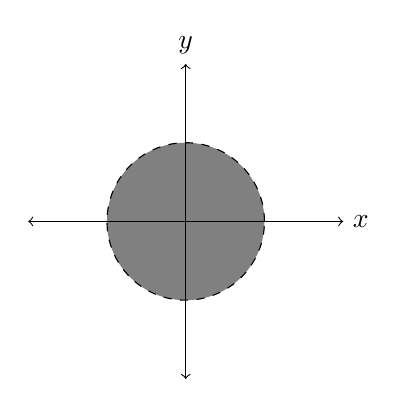
\begin{tikzpicture}
\draw[dashed, fill = gray] (0,0) circle (1);
\draw[<->] (-2,0) -- (2,0);
\node[anchor = west] at (2,0) {$x$};
\draw[<->] (0,-2) -- (0,2);
\node[anchor = south] at (0,2) {$y$};
\end{tikzpicture}
\end{image}

The set $\{(x,y)\;:\;x^2+y^2\leq 1\}\subset\mathbb{R}^2$ is both closed and bounded, hence compact.

\begin{image}
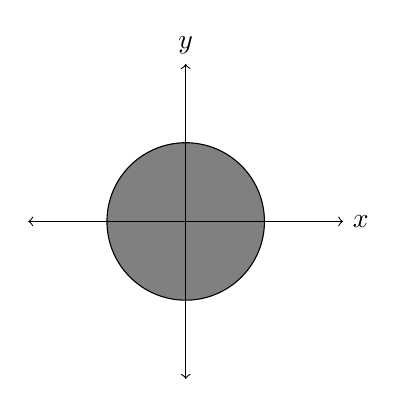
\begin{tikzpicture}
\draw[fill = gray] (0,0) circle (1);
\draw[<->] (-2,0) -- (2,0);
\node[anchor = west] at (2,0) {$x$};
\draw[<->] (0,-2) -- (0,2);
\node[anchor = south] at (0,2) {$y$};
\end{tikzpicture}
\end{image}

The set $\{(x,y)\;:\;x^2+y^2\geq 1\}\subset\mathbb{R}^2$ is  closed but not bounded. Hence it is not compact.

\begin{image}
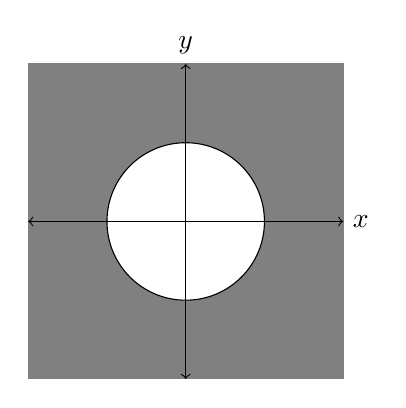
\begin{tikzpicture}
\draw[color = gray, fill = gray] (-2,-2) -- (-2,2) -- (2,2) -- (2,-2);
\draw[fill = white] (0,0) circle (1);
\draw[<->] (-2,0) -- (2,0);
\node[anchor = west] at (2,0) {$x$};
\draw[<->] (0,-2) -- (0,2);
\node[anchor = south] at (0,2) {$y$};
\end{tikzpicture}
\end{image}

\end{example}

\begin{problem}
Sketch each region, and determine if it is closed, bounded, and/or compact.

$\{(x,y)\}\;:\;-1\leq x\leq 1\}$
\begin{selectAll}
\choice[correct]{closed}
\choice{bounded}
\choice{compact}
\end{selectAll}

$\{(x,y)\}\;:\;-1\leq y\leq 1\}$
\begin{selectAll}
\choice[correct]{closed}
\choice{bounded}
\choice{compact}
\end{selectAll}

$\{(x,y)\}\;:\;-1\leq x\leq 1\text{ and }-1\leq y\leq 1\}$
\begin{selectAll}
\choice[correct]{closed}
\choice[correct]{bounded}
\choice[correct]{compact}
\end{selectAll}

$\{(x,y)\}\;:\;x^2-1\leq y\leq 1-x^2\}$
\begin{selectAll}
\choice[correct]{closed}
\choice[correct]{bounded}
\choice[correct]{compact}
\end{selectAll}

$\{(x,y)\}\;:\;-x^2\leq y\leq x^2\}$
\begin{selectAll}
\choice[correct]{closed}
\choice{bounded}
\choice{compact}
\end{selectAll}

\end{problem}

\section*{Extreme Value Theorem}

As in the single variable case, as long as we have a continuous function over a compact region, there is guaranteed to be an absolute maximum and absolute minimum. Furthermore, these will always occur either at critical points, or on the boundary.

\begin{theorem}
(Extreme Value Theorem) Let $f:X\rightarrow\mathbb{R}$ be a continuous function on a compact region $X\subset \mathbb{R}^n$. Then $f$ has both an absolute maximum and an absolute minimum over $X$.

 Furthermore, if $f$ has an absolute maximum or absolute minimum at $\vec{a}$, then either $\vec{a}$ is a critical point of $f$ in $X$, or $\vec{a}$ is on the boundary of $X$.
\end{theorem}

Because of this theorem, we can follow the steps below to optimize a continuous function $f$ on a compact region $X$.
\begin{enumerate}
\item Find the critical points of $f$ in $X$, and find the value of $f$ at each of these points.
\item Find the absolute maximum and absolute minimum of $f$ on the boundary of $X$.
\item Of the values from steps 1 and 2, the largest value is the absolute maximum of $f$ over $X$, and the smallest value is the absolute minimum of $f$ over $X$.
\end{enumerate}

\begin{example}
We'll find the absolute maximum and minimum values of $f(x,y)= x^2-xy+y^2$ on $D=\{(x,y)\;:\;x^2+y^2\leq 1\}\subset \mathbb{R}^2$.

\begin{image}
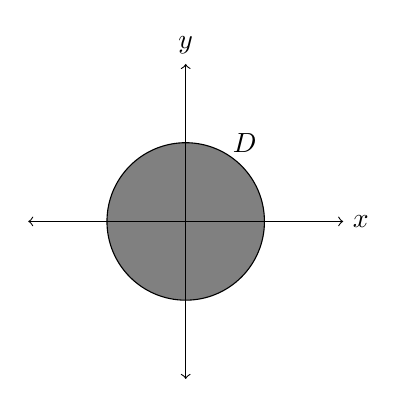
\begin{tikzpicture}
\draw[fill = gray] (0,0) circle (1);
\draw[<->] (-2,0) -- (2,0);
\node[anchor = west] at (2,0) {$x$};
\draw[<->] (0,-2) -- (0,2);
\node[anchor = south] at (0,2) {$y$};

\node[anchor = south] at (.75,.75) {$D$};
\end{tikzpicture}
\end{image}

First, note that $f$ is continuous, and $D$ is a compact region, so $f$ has an absolute maximum and an absolute minimum over $D$, and each occurs either at a critical point or on the boundary of $D$.

We first find the critical points of $f$, by finding where the gradient is $\vec{0}$.
\[
\nabla f(x,y) = \answer{(2x-y, -x+2y)}
\]
Solving for where $\nabla f(x,y) = (0,0)$, we obtain the only critical point,
\[
(x,y) = \answer{(0,0)}.
\]
The value of $f$ at this critical point is $\answer{0}$.

Next, we need to find the maximum and minimum values of $f$ on the boundary of $X$, which is the unit circle. In order to do this, we parametrize the unit circle,
\[
\vec{x}(t) = (\cos(t),\sin(t)),
\]
for $t\in [0,2\pi]$. Substituting this into $f$, we can find the maximum and minimum of $f$ on the boundary of $X$ by finding the maximum and minimum of the single variable function
\begin{align*}
g(t) &= \cos^2 t - \cos(t)\sin(t) + \sin^2t\\
&= 1-\cos(t)\sin(t)
\end{align*}
over $[0,2\pi]$. To optimize this function, we follow the closed interval method for single variable functions. Differentiating $g$, we have
\begin{align*}
g'(t) &= \sin^2(t) - \cos^2(t)\\
&= -\cos(2t).
\end{align*}
Solving $g'(t)=0$ for $t$, the critical points in the interval $[0,2\pi]$ are $t=\frac{\pi}{4}$, $t =\frac{3\pi}{4}$, $t = \frac{5\pi}{4}$, and $t = \frac{7\pi}{4}$ . The values of $g$ at these points are
\begin{align*}
g\left(\frac{\pi}{4}\right) = \frac{1}{2},\\
g\left(\frac{3\pi}{4}\right) = \frac{3}{2},\\
g\left(\frac{5\pi}{4}\right) = \frac{1}{2},\\
g\left(\frac{7\pi}{4}\right) = \frac{3}{2}.\\
\end{align*}
The values of $g$ at the endpoints, $t=0$ and $t=2\pi$, are
\begin{align*}
g(0) &= 1,\\
g(2\pi) &= 1.
\end{align*}
Comparing all of these values, we see that the absolute maximum of $g$ is $\frac{3}{2}$, and this occurs when $t=\frac{3\pi}{4}$ and when $t=\frac{7\pi}{4}$. These correspond to the points $\left(\frac{-\sqrt{2}}{2},\frac{\sqrt{2}}{2}\right)$ and $\left(\frac{\sqrt{2}}{2},\frac{-\sqrt{2}}{2}\right)$ on the boundary of $D$. The absolute minimum of $g$ is $\frac{1}{2}$, and this occurs when $t=\frac{\pi}{4}$ and when $t=\frac{5\pi}{4}$. These correspond to the points $\left(\frac{\sqrt{2}}{2},\frac{\sqrt{2}}{2}\right)$ and $\left(\frac{-\sqrt{2}}{2},\frac{-\sqrt{2}}{2}\right)$ on the boundary of $D$.

Now, considering the values of $f$ at the critical points and on the boundary of $X$, we see that the absolute maximum of $f$ is $\frac{3}{2}$ and this occurs at $\left(\frac{-\sqrt{2}}{2},\frac{\sqrt{2}}{2}\right)$ and $\left(\frac{\sqrt{2}}{2},\frac{-\sqrt{2}}{2}\right)$. The absolute minimum of $f$ is $0$ and this occurs at $(0,0)$.

\begin{image}

\includegraphics[width=\textwidth]{CalcPlot3D-abs_extrema}
\end{image}
\end{example}




\end{document}